\documentclass[aspectratio=169,11pt]{beamer}

\usepackage[T1]{fontenc}
\usepackage[utf8]{inputenc}
\usepackage{lmodern}
\usepackage{tikz}
\usetikzlibrary{positioning,arrows.meta,shapes.geometric,fit}
\usepackage{booktabs}
\usepackage{array}

% ---------- Palette ----------
\definecolor{thgablue}{HTML}{003C7C}
\definecolor{accentred}{HTML}{E5000F}
\definecolor{ink}{HTML}{15202B}
\definecolor{muted}{HTML}{5C6773}
\definecolor{soft}{HTML}{F3F6F9}
\definecolor{linegray}{HTML}{D9E0E6}

\setbeamercolor{normal text}{fg=ink,bg=white}
\setbeamercolor{structure}{fg=thgablue}
\setbeamercolor{frametitle}{fg=thgablue,bg=white}
\setbeamercolor{title}{fg=white}
\setbeamercolor{subtitle}{fg=white}
\setbeamercolor{author}{fg=white}
\setbeamercolor{date}{fg=white}
\setbeamercolor{block title}{fg=white,bg=thgablue}
\setbeamercolor{block body}{fg=ink,bg=soft}
\setbeamertemplate{navigation symbols}{}
\setbeamertemplate{footline}{%
  \leavevmode\hbox{%
    \begin{beamercolorbox}[wd=.82\paperwidth,ht=2.6ex,dp=1ex,leftskip=1.1em]{author in head/foot}%
      \color{muted}\scriptsize Chess Club Tournament \& Rating Manager
    \end{beamercolorbox}%
    \begin{beamercolorbox}[wd=.18\paperwidth,ht=2.6ex,dp=1ex,rightskip=1.1em plus1fil]{author in head/foot}%
      \hfill\color{muted}\scriptsize \insertframenumber/\inserttotalframenumber
    \end{beamercolorbox}%
  }%
}
\setbeamertemplate{frametitle}{%
  \vspace{0.45em}
  \begin{beamercolorbox}[wd=\paperwidth,leftskip=0.6cm,sep=0.2cm]{frametitle}
    \usebeamerfont{frametitle}\Large\bfseries\insertframetitle
  \end{beamercolorbox}
  \vspace{-0.3em}
  \hspace{0.6cm}\color{accentred}\rule{1.15cm}{2.2pt}
}

\newcommand{\bigidea}[1]{\begin{center}\color{thgablue}\bfseries\Large #1\end{center}}
\newcommand{\tagpill}[1]{\tikz[baseline=(X.base)]\node[rounded corners=3pt,fill=soft,inner xsep=7pt,inner ysep=3pt,text=thgablue,font=\small\bfseries] (X) {#1};}

\title{Chess Club Tournament \& Rating Manager}
\subtitle{Self-hosted tournament workflow with automatic Elo tracking}
\author{Yahya El Idrissi}
\date{THGA Bochum - Introduction to DBMS}

\begin{document}

% ---------- 1: Title ----------
{
\setbeamertemplate{footline}{}
\begin{frame}[plain]
  \begin{tikzpicture}[remember picture,overlay]
    \fill[thgablue] (current page.south west) rectangle (current page.north east);
    \fill[accentred] (current page.south west) rectangle ([xshift=0.16cm]current page.north west);
    \fill[white,opacity=.07] ([xshift=8.0cm,yshift=-1.0cm]current page.north west) circle (3.6cm);
    \fill[white,opacity=.05] ([xshift=12.2cm,yshift=1.0cm]current page.south west) circle (2.8cm);
  \end{tikzpicture}
  \vspace{1.0cm}
  {\color{white}\Huge\bfseries Chess Club Tournament\\[0.12cm]\& Rating Manager\par}
  \vspace{0.45cm}
  {\color{white!85}\Large Self-hosted tournament workflow with automatic Elo tracking\par}
  \vfill
  {\color{white}\large Yahya El Idrissi\par}
  \vspace{0.12cm}
  {\color{white!75}\normalsize THGA Bochum - Introduction to DBMS\par}
  \vspace{0.6cm}
\end{frame}
}

% ---------- 2: Problem / Product ----------
\begin{frame}{From scattered work to one workflow}
\vspace{0.15cm}
\begin{columns}[T,onlytextwidth]
  \column{0.47\textwidth}
    \begin{block}{Typical small-club workflow}
      \vspace{0.15cm}
      \begin{itemize}\setlength\itemsep{0.45em}
        \item Player lists in spreadsheets
        \item Tournament data stored separately
        \item Elo ratings calculated manually
        \item Standings assembled after each round
      \end{itemize}
      \vspace{0.05cm}
    \end{block}
  \column{0.49\textwidth}
    \begin{block}{This project}
      \vspace{0.15cm}
      \begin{itemize}\setlength\itemsep{0.45em}
        \item One desktop application
        \item One PostgreSQL database
        \item Automatic Elo + rating history
        \item Standings with Buchholz tiebreak
      \end{itemize}
      \vspace{0.05cm}
    \end{block}
\end{columns}
\vspace{0.4cm}
\bigidea{Goal: make the tournament workflow simple, traceable and self-hosted.}
\end{frame}

% ---------- 3: Workflow ----------
\begin{frame}{Core product workflow}
\vspace{0.55cm}
\begin{center}
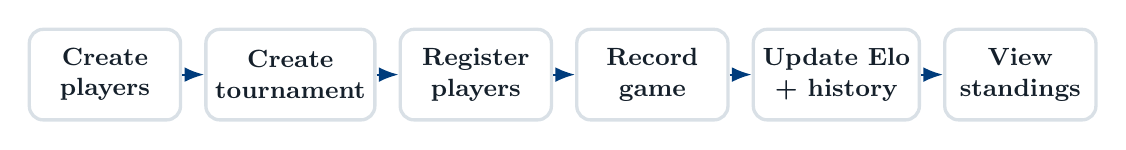
\begin{tikzpicture}[
  node distance=0.28cm,
  flowbox/.style={rounded corners=5pt,draw=linegray,very thick,fill=white,minimum width=1.92cm,minimum height=1.15cm,align=center,font=\small\bfseries,text=ink},
  arr/.style={-{Latex[length=2.5mm]},thick,draw=thgablue}
]
\node[flowbox] (p) {Create\\players};
\node[flowbox,right=of p] (t) {Create\\tournament};
\node[flowbox,right=of t] (r) {Register\\players};
\node[flowbox,right=of r] (g) {Record\\game};
\node[flowbox,right=of g] (e) {Update Elo\\+ history};
\node[flowbox,right=of e] (s) {View\\standings};
\draw[arr] (p) -- (t);
\draw[arr] (t) -- (r);
\draw[arr] (r) -- (g);
\draw[arr] (g) -- (e);
\draw[arr] (e) -- (s);
\end{tikzpicture}
\end{center}
\vspace{0.8cm}
\begin{center}
  \tagpill{Live demo follows this exact flow}\qquad
  \tagpill{Automatic pairing is intentionally out of scope}
\end{center}
\end{frame}

% ---------- 4: Architecture ----------
\begin{frame}{Architecture}
\vspace{0.35cm}
\begin{center}
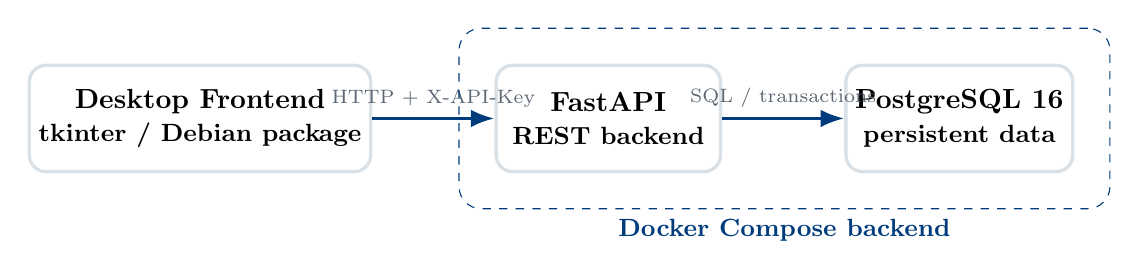
\begin{tikzpicture}[
  box/.style={rounded corners=6pt,draw=linegray,very thick,fill=white,minimum width=2.85cm,minimum height=1.35cm,align=center,font=\bfseries},
  arr/.style={-{Latex[length=3mm]},very thick,draw=thgablue},
  note/.style={font=\scriptsize,text=muted,align=center}
]
\node[box] (fe) {Desktop Frontend\\\small tkinter / Debian package};
\node[box,right=1.55cm of fe] (api) {FastAPI\\\small REST backend};
\node[box,right=1.55cm of api] (db) {PostgreSQL 16\\\small persistent data};
\draw[arr] (fe) -- node[above,note] {HTTP + X-API-Key} (api);
\draw[arr] (api) -- node[above,note] {SQL / transactions} (db);
\node[draw=thgablue,dashed,rounded corners=8pt,fit=(api)(db),inner sep=0.45cm,label={[text=thgablue,font=\small\bfseries]below:Docker Compose backend}] {};
\end{tikzpicture}
\end{center}
\vspace{0.85cm}
\begin{columns}[T,onlytextwidth]
  \column{0.48\textwidth}
  \textbf{Configurable at startup}\par
  \small API URL and API key are entered in a connection dialog.
  \column{0.48\textwidth}
  \textbf{Self-hosted by design}\par
  \small The application can run against the local backend or a remote server.
\end{columns}
\end{frame}

% ---------- 5: Data + logic ----------
\begin{frame}{Database and critical logic}
\vspace{0.25cm}
\begin{columns}[T,onlytextwidth]
  \column{0.43\textwidth}
  \begin{block}{7-table relational model}
    \small
    \begin{tabular}{@{}ll@{}}
      \textbf{Core} & player, tournament, round \\
      \textbf{N:M} & registration \\
      \textbf{Games} & game, opening \\
      \textbf{History} & rating\_history \\
    \end{tabular}
  \end{block}
  \vspace{0.25cm}
  \small
  \textbf{Database-level checks}\par
  Foreign keys, valid results, unique rounds, and white $\neq$ black.

  \column{0.52\textwidth}
  \begin{block}{Recording one game}
    \small
    \begin{enumerate}\setlength\itemsep{0.25em}
      \item Validate round + registrations
      \item Insert game result
      \item Calculate both Elo ratings ($K=20$)
      \item Update both players
      \item Insert two history entries
    \end{enumerate}
  \end{block}
  \vspace{0.25cm}
  \small\textbf{One transaction:} either every step succeeds, or the operation rolls back.
\end{columns}
\end{frame}

% ---------- 6: Live demo ----------
\begin{frame}{Live demo: from empty database to standings}
\vspace{0.15cm}
\begin{columns}[T,onlytextwidth]
  \column{0.55\textwidth}
    \begin{block}{Demo data}
      \small
      \begin{tabular}{>{\bfseries}p{2.2cm}p{4.5cm}}
        Players & Alice (1200), Bob (1200) \\
        Tournament & Club Open 2026, 1 round \\
        Registration & Alice + Bob \\
        Game & Alice - Bob, C50, 1-0 \\
      \end{tabular}
    \end{block}
  \column{0.40\textwidth}
    \begin{block}{What to verify}
      \small
      \begin{itemize}\setlength\itemsep{0.38em}
        \item Players stored
        \item Elo changes automatically
        \item Rating history grows
        \item Standings update
        \item Buchholz is available
      \end{itemize}
    \end{block}
\end{columns}
\vspace{0.4cm}
\bigidea{Next: run the application live.}
\end{frame}

% ---------- 7: Delivery / closing ----------
\begin{frame}{Delivered as a complete project}
\vspace{0.2cm}
\begin{columns}[T,onlytextwidth]
  \column{0.49\textwidth}
  \begin{block}{Engineering quality}
    \small
    \begin{itemize}\setlength\itemsep{0.35em}
      \item API endpoint tests
      \item Database schema + seed smoke test
      \item Docker Compose backend smoke test
      \item Debian frontend package build
      \item LaTeX documentation build
    \end{itemize}
  \end{block}
  \column{0.47\textwidth}
  \begin{block}{Possible next steps}
    \small
    \begin{itemize}\setlength\itemsep{0.35em}
      \item Automatic pairings
      \item Edit / delete workflows
      \item User accounts + roles
      \item More tournament formats
      \item Richer reporting / export
    \end{itemize}
  \end{block}
\end{columns}
\vspace{0.28cm}
\bigidea{One self-hosted workflow for players, games, ratings and standings.}
\end{frame}

\end{document}
